\chapter{Literature review}

\section{Review paper 1 - Prototype CNC machine design}

\subsection{CNC Module introduction}
The Computer Numeric Control (CNC) is a technology which aims to generate, parse and execute sequential action. It helps for the development of small and big sized CNC machines, based on a system with the capability of communication through a communication bus. It is also required electronic devices to run a CNC machine like controller circuit, as well, a software developed in LabVIEW to establish the communication between the machine and the computer. The main objective of this work is the development of a machine which allows future use for PCB track designing with better efficiency than traditional methods.A CNC prototype machine was designed, with three-axis movement, with 300 mm of length both X and Y axes and 10 mm of the length Z-axis. \par

CNC Machines are often used in metal machining, like drilling, milling etc. This kind of machine consists usually of a servo mechanism controlled by a computer, a high-speed spindle and dedicated tools. This servo mechanism can be realized in a closed-loop fashion, using servo controllers driving DC or synchronous AC machines, or open-loop fashion, using stepper motors. small loads required an open-loop system for a better fit. Therefore, industrial-sized machines do not, in general, use open-loop machines. \par

The machine is based on the removal of the material of a workpiece. Nowadays, there are machines with six or more axes, which allow the machining of pieces which can handle high levels of complexity that is feasible by all other means.


\subsection{Use of CNC machine}
CNC machines can be used in many different ways, including (but not restricted to):

\begin{enumerate}
    \item Making circuits boards - They are used to make printed circuit boards for different products
    \item Making enclosures - The different types of CNC machines like laser cutters, mills and lathes use some parts to make enclosures. Sticker cutters are also used to make decorations for enclosures.
    \item For Computer Integrated Manufacturing - They are programmed in a specific way according to instructions, and this can save hundreds of thousands of hours of manual programming.
\end{enumerate}

The CNC machine is used in many different industries, including:

\begin{enumerate}
    \item Agriculture - The agriculture industry requires reliable, high-quality production of machine parts and other products.
    \item Transportation - Some vehicle parts like gears, brakes, pins and shafts need precise CNC machining in their manufacturing.
    \item Firearms - CNC machines are needed to create complex barrels, plates and triggers, among other things.
\end{enumerate}

\section{Review paper 2 - Automatic mini CNC machine for drawing and drilling}

\subsection{Methodology}
The G code is interfaced with an Arduino CNC based controller by software which is used to convert into equivalent controller instructions. Hence it acts as an interfacing module between PC to Controller. This code is further passed to the stepper motor by easy drivers which convert the code and as per instructions the stepper motor moves. We need three axes X, Y, Z which operates as follows X stepper motor moves left and right Y stepper motor moves front and back and Z stepper motor up and down as per given dimensions these axes will move on.

\subsection{G codes and M codes}
PC G code is a converted instruction form of programming language which defines instructions on where to move, how fast to move with the path.

\subsection{CNC shield}
\begin{itemize}
    \item GRBL 0.8c compatible. (Open supply microcode that runs on associate degree Arduino UNO that turns G-code commands into stepper signal.)
    \item 4-Axis support (X, Y, Z, A-Can duplicate X, Y, Z or do a full 4th axis with custom firmware using pins D12 and D13)
    \item 2 x finish stops for every axis (6 in total)
    \item Spindle enable and direction
    \item Coolant enable
    \item Uses removable Pololu A4988 compatible stepper drivers. (A4988, DRV8825 and others)
    \item Jumpers to line the Micro stepping for the stepper drivers. (Some drivers just like the DRV8825 will do up to 1/32 micro-stepping )
    \item Compact design
    \item Stepper Motors may be connected with four pin Molex connectors.
    \item Runs on 12-36V DC. (At the instant solely the Pololu DRV8825 drivers will handle up to 36V thus please take into account the operation voltage once powering the board.
\end{itemize}

\subsection{Generic block diagram}

\begin{figure}[h]
    \centering
    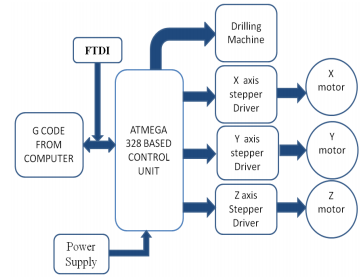
\includegraphics{Chapter_2/paper_block_diagram.png}
    \caption{Block diagram of the CNC machine developed in the paper}
    \label{fig:block_diagram}
\end{figure}

\subsection{Stepper motor and associated parts}

\subsubsection*{NEMA 17 stepper motor}
Stepper motors are sort of DC motors that move in increments or steps, they move at a legendary interval for every pulse of power. These pulses of power are provided by a motor driver and are referred to as a step. As every step moves a legendary distance it makes them handy devices for repeatable positioning. Stepper motors are usually used on CNC Machines such as 3D Printers, Laser Cutters, CNC Routers.


\subsection{Micro controller requirements}

\subsubsection*{Micro controller - Arduino UNO r3}
The Arduino UNO R3 could be a microcontroller board supporting the ATmega328. It has fourteen digital input/output pins (of that vi may be used as PWM outputs), 6 analog inputs, a 16 MHz crystal oscillator, a USB connection, a power jack, an ICSP header, and a reset button. It contains everything required to support the microcontroller; merely connect it to a PC with a USB cable or power it with an AC-to-DC adapter or battery to induce power. \par

The Uno differs from all preceding boards in that it doesn't use the FTDI USB-to-serial driver chip. Instead, it options the Atmega16U2 (Atmega8U2 up to version R2) programmed as a USB-to-serial converter.
Revision a pair of the Uno board features a resistance propulsion the 8U2 HWB line to ground, making it easier to put into DFU.

Revision three of the board has the subsequent new features:

\begin{itemize}
    \item 1.0 pinout: added SDA and SCL pins that are near to the AREF pin and two other new pins placed near the RESET pin, the IOREF that allow the shields to adapt to the voltage provided from the board. In future, shields are compatible with the board that uses the AVR, which operates with 5V and with the Arduino Due that operate with 3.3V. The other could be a not connected pin, that is reserved for future functions.
    \item Stronger RESET circuit.
    \item Atmega 16U2 replaced the 8U2.
\end{itemize}


\section{Review paper 3 - CNC fabrication and user manual} \label{Sec:3}

This reference instead of being a paper happens to be a detailed user manual regarding how one should use a typical CNC machine for PCB prototyping purposes. It starts off on similar lines of needs and requirements as the CNC machine being developed by the authors of this report. It then goes on to explain various software aspects of PCB design followed by which it describes what are the standard and special procedures used in CNC machines such as moving the tooltip to the origin/soft - home position, calibration of various important parts to name a few. \par

A BYO PCB prototyping machine capable of developing both through hole and Surface Mount Technology on single sided and double sided PCB boards has been used as a standard reference throughout the manual. Following is a detailed description of  only the important and relevant sections of the concerned manual.


\begin{figure}[h]

\begin{subfigure}{0.5\textwidth}
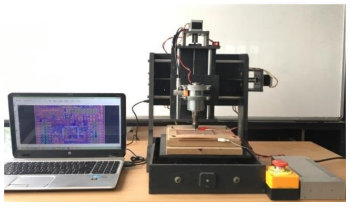
\includegraphics[width=0.9\linewidth, height=6cm]{Chapter_2/mechanical_setup.PNG}
\caption{Mechanical Setup of the Machine}
\label{fig:subim1}
\end{subfigure}
\begin{subfigure}{0.5\textwidth}
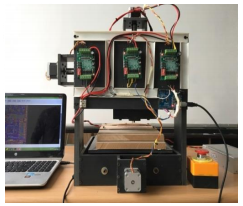
\includegraphics[width=0.9\linewidth, height=6cm]{Chapter_2/electronics_assembly.PNG} 
\caption{Electronics hardware assembly}
\label{fig:subim2}
\end{subfigure}

\caption{The PCB prototyping machine as described in the reference manual}
\label{fig:paper_cnc_machine}
\end{figure}


\subsection{Layers of a PCB copper clad}

Understanding PCB composition in hindsight is simply understanding how layers of a PCB are stacked over one other and what is the significance of each layer. The most important layer(s) of the PCB copper cladding is the copper layers themselves. These are the layers through which the intended electrical signals pass depending on the application. The copper layers sandwich a layer which is usually the thickest layer in a copper cladding. It is an insulating layer called the substrate. Depending on the application the substrate layer could be made of various materials of various thicknesses. The most common ones are FR4 which is a NEMA grade designation for glass-reinforced epoxy laminate material and FR2 which is a phenolic cotton paper. FR2 is very common in single-sided PCBs in consumer electronics while FR4 is universal in multi-layer PCBs and in general. \par


\begin{figure}[h]
    \centering
    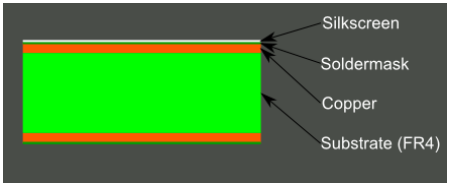
\includegraphics{Chapter_2/pcb_layers.PNG}
    \caption{The layers of a double-sided PCB}
    \label{fig:pcb_layers}
\end{figure}

Now to insulate and protect the copper layers they are covered by a thin lacquer-like material called the solder mask. This layer is responsible for the characteristic “green” colour of PCBs or whatever colour (red, blue etc.) they are supposed to have. Then the final set of top and bottom layers of a PCB is the silkscreen which has a look and feels similar to ink and can be used to add texts and logos to a PCB. Following is an illustration of the various layers of a double-sided PCB copper cladding. \par

% add table for eagle layers %


The PCB designer has access to all the layers at any given instant of time during the development of a particular PCB. For the designer using the EAGLE software, a palette of colours (as shown below) is used to represent the various layers of a PCB. They can be toggled according to the convenience of the designer by going into the layer settings of the board and clicking the layer number to toggle it in view. 

\subsection{CAM processing}

CAD/CAM processing belongs to a much larger set/group of processes used in the industry collectively called machining. \textbf{Machining} is any of the varied processes during which a bit of staple is dug into a desired final shape and size by a controlled material removal process. The common theme of machining remains as controlled material removal which could be either additive or subtractive in nature. As the words themselves suggest additive manufacturing shall add material to the original raw material while subtractive manufacturing refers to the opposite.  \par

Nowadays, all machining has been converted into OR is exclusively carried out by Computer Numerical Control (CNC). Computer-Aided Design (CAD) and Computer-Aided Manufacturing (CAM) fall under this much larger umbrella of  “CNC jobs”. This paper explains how to use the CAM processor present in the EAGLE software to generate a CNC job corresponding to a given board file. The same CAM processor can be used to generate  “Gerber” files for all the layer(s) of a given PCB as well as “Excellon” files for drilling purposes of the concerned  PCB. These types of files come under the much larger umbrella of PCB NC formats which manage to convey routing and drilling information to the concerned CNC machine. \par

Later the Gerber files generated are sent to “FlatCAM” which is a CAM processing software responsible for generating CNC jobs from Gerber files obtained from any PCB CAD program. It does the additional job of generating corresponding “g codes” for routing purposes and allowing the user to edit the same.


\subsection{Special procedures}

Several challenges arise when designing complex PCB designs; these challenges could range from manufacturing multilayered boards to working on uneven surfaces. The associated software for a given CNC machine and some simple procedures help the users overcome these challenges. Few of those which were discussed in this paper are described below.

\subsubsection*{Auto levelling}
It is not uncommon to have inconsistent traces in larger PCBs while using a CNC based milling machine. Such inconsistencies arise due to minor height variations of the surface on which the PCB is kept (“wasteboard”) OR the PCB by itself could be bent or warped. It should be noted that even minor height variations of about 1 mm could change the groove width by about 0.672 mm.  To overcome this problem we need specialised software called auto levelling software. By definition, Auto-levelling is a process that tries to \textbf{compensate} for height differences instead of \textbf{trying to prevent them.} \par

Auto levelling software depending on their sophistication may approach this problem in different ways and use different forms of sensory data to solve the problem. The most common way to approach this problem is by dividing the entire PCB into uniform geometrical grids. This gives specific sampling positions which could be probed to get an overall idea of the non-uniformities of the surface. For e.g. a 40 x 40 mm surface could be divided into 100 grids of 4 x 4 mm and the surface at the centre of the grids is always probed.  Probing the height of a PCB locally (i.e. in every grid) is typically done by slowly lowering an end mill until an \textbf{electric connection is made between the end mill and board’s copper layer}. All these things are usually automated by the software. However, if it is not the case the designer has to design compensation algorithms on their own. \par

First, all the collected data is accumulated in a single file called the probe file. The generated G code and this file are superimposed and fed to the software. The software now tries to fit a \textit{quadratic surface} (say of the form $f(x^{2},y^{2})$) on the probe data and accordingly adjusts the G code in the vertical direction. This adjusted G code can be fed into the CNC machine like any other G code file thereby eliminating any problems that may result from an uneven or warped surface.

\begin{figure}[h]
    \centering
    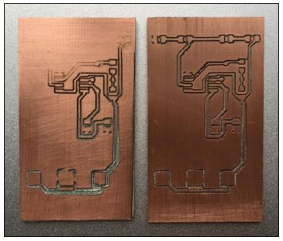
\includegraphics{Chapter_2/with_and_without_autolevel.PNG}
    \caption{Showing the making of PCB board with and
without the use of Autoleveller on a skewed platform}
    \label{fig:with_without_auto}
\end{figure}

\subsubsection*{Copper area clear}

With RF circuit PCBs or any PCB, in general, comes the problem of clearing large areas of unwanted copper traces which is just unwanted core load. The manual explains how to use the various properties available under the “Gerber object” tab to eliminate unwanted copper traces. After specifying the margin dimensions, a boundary (called the “bounding box”) is created. A geometric subtraction of the Gerber object from the boundary will give rise to another Gerber object which doesn’t have areas with copper on them. A number of polygons constitute this newly formed Gerber object. The user gets to choose which Gerber object to keep and what not to. To do so the correct tool dimensions with its specifications are selected and the concerned/desired polygon is painted. “Painting” refers to covering the whole polygon with the tool paths (whose specifications were selected within the previous step). In this manner, all unwanted copper load can be removed from any type of PCB.

\begin{figure}[ht]
\begin{subfigure}{0.5\textwidth}
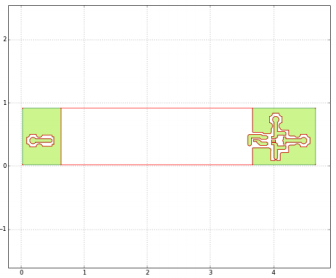
\includegraphics[width=\linewidth, height=6cm]{Chapter_2/copper_area_clear_1.PNG}
\caption{Geometry object with polygons covering the areas without copper}
\label{fig:copper_clear_1}
\end{subfigure} 
\begin{subfigure}{0.5\textwidth}
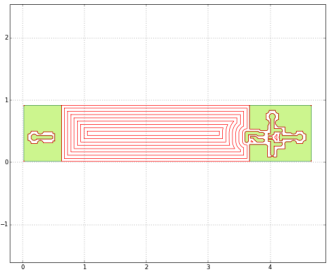
\includegraphics[width=0.9\linewidth, height=6cm]{Chapter_2/copper_area_clear 2.PNG} 
\caption{New Geometry Object with the desired tool paths that can overlap too.}
\label{fig:copper_clear_2}
\end{subfigure}

\caption{The software steps during the procedure of \textit{copper clear}}
\label{fig:copper_clear}
\end{figure}

\subsubsection*{Board cutout}

PCBs need to be cut out from much larger and blank copper claddings, otherwise, we shall incur large material wastage in terms of area and cost. The FlatCAM software allows the user to do so by selecting the board cutout tab after choosing a Gerber file. The desired margin (dimension) is selected which tells how far the cutout boundary is from any element of the Gerber source of the PCB. After this “gaps” can be selected for the cutout in terms of their dimensions and their number. It is always recommended to have gap size twice the diameter of the tooltip. FlatCAM allows two gaps (either on top and bottom OR left and right) or four gaps for a given PCB. Once, this step is complete, just like the previous procedure the geometry for the tool path is generated. A CNC job is created from this geometry just like any other geometry and now the job is ready to be processed.  Hence, this feature allows precise cutting of a PCB from its larger blank cladding once the main CNC job is done.

\begin{figure}[h]
    \centering
    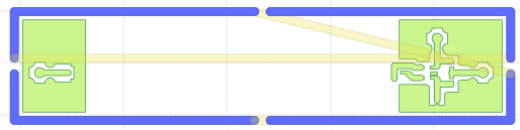
\includegraphics{Chapter_2/board_cutout.PNG}
    \caption{Typical CNC job corresponding to a \textit{board cutout}}
    \label{fig:board_cutout}
\end{figure}


\subsection{Computing resolution and accuracy}
A lot of experimentation needs to be carried out to verify the practicality of the CNC machine. A typical experimentation procedure needs to be carried out to find out the wire width and resolution capabilities of the PCB. The next part is computing the resolution for SMT fabrication purposes. Both the techniques have been briefly discussed in the manual.

\subsubsection*{Computing wire width and resolution}
To find out the level of resolution while tracing out or engraving wires, a good way is to make a very simple PCB consisting of wires of various widths, to be precise, in decreasing order. The wire of largest possible width (available in the schematic design software) is made followed by the next largest and so on and so forth until the wire of minimum possible width possible in the schematic design software is designed. Now the G codes corresponding to this sample PCB are sent to the CNC machine before milling the same. \par

After the PCB tracks have been engraved on to the copper cladding by the CNC machine, the absolute deviation between the width of the actual engraved tracks and input width for the concerned track provided as input from the software is computed. (Insert equation) This denotes the resolution of the CNC machine. It should be noted that it is not compulsory to compute the absolute deviation, positive and negative deviations are both valid. To carry out this measurement, a handheld microscope is a suitable instrument. For the CNC machine in question, the wire of the smallest width that could be fabricated was found out to be 0.2 mm with an allowable deviation of -0.012 mm.

\begin{figure}[h]
    \centering
    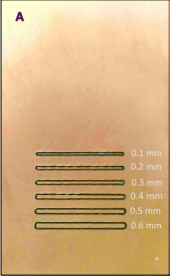
\includegraphics{Chapter_2/test_widths.PNG}
    \caption{PCB fabricated with sample wires of varying widths}
    \label{fig:wire_widths}
\end{figure}


\subsubsection*{Resolution of SMT}

Various standard and commonly used SMT packages were fabricated by the CNC machine. It was found out that the minimum pitch size of an SMT that could be fabricated was about as low as 0.3 mm. A handheld USB microscope was used for the purpose of measurements in each case.

\begin{figure}[h]
    \centering
    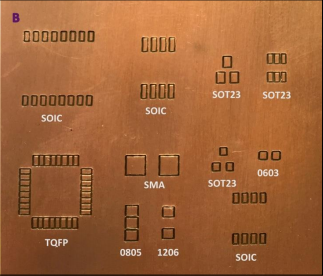
\includegraphics{Chapter_2/test_smt.PNG}
    \caption{PCB fabricated with SMTs of varying footprints}
    \label{fig:smts}
\end{figure}
